\documentclass[11pt]{article}
\usepackage{Fall23/classTools}
\usepackage{xcolor}
\usepackage{graphicx}
\usepackage{amsfonts}
\usepackage{amsmath}
\usepackage{minted}
\def\draft{1}

\begin{document}
\psHeader{0}{Wed 2023-09-13 (11:59PM)}

 \newcommand{\children}{\mathit{children}}
 \newcommand{\parent}{\mathit{parent}}
 
\begin{enumerate}
\item (Binary Trees) 

 \begin{enumerate}
 \item \label{part:calculatesizes} (recursive programming)
 Write a recursive program \texttt{calculate\_sizes} that given a vertex \btv\ of a binary tree \treeT, calculates the sizes of all of the subtrees rooted at descendents of \btv.  After running your program on \texttt{T.root}, every vertex \btv\ in \treeT\ should have \texttt{v.size} set to the size of the subtree rooted at \btv. (Recall that the size attributes are initialized to \texttt{None}.)  We call the resulting tree a {\em size-augmented} tree.
 
For example, if \treeT\  is the  tree shown above, 
then calling \texttt{calculate\_sizes(T.root)} should modify  \treeT\ to be the following size-augmented tree:

 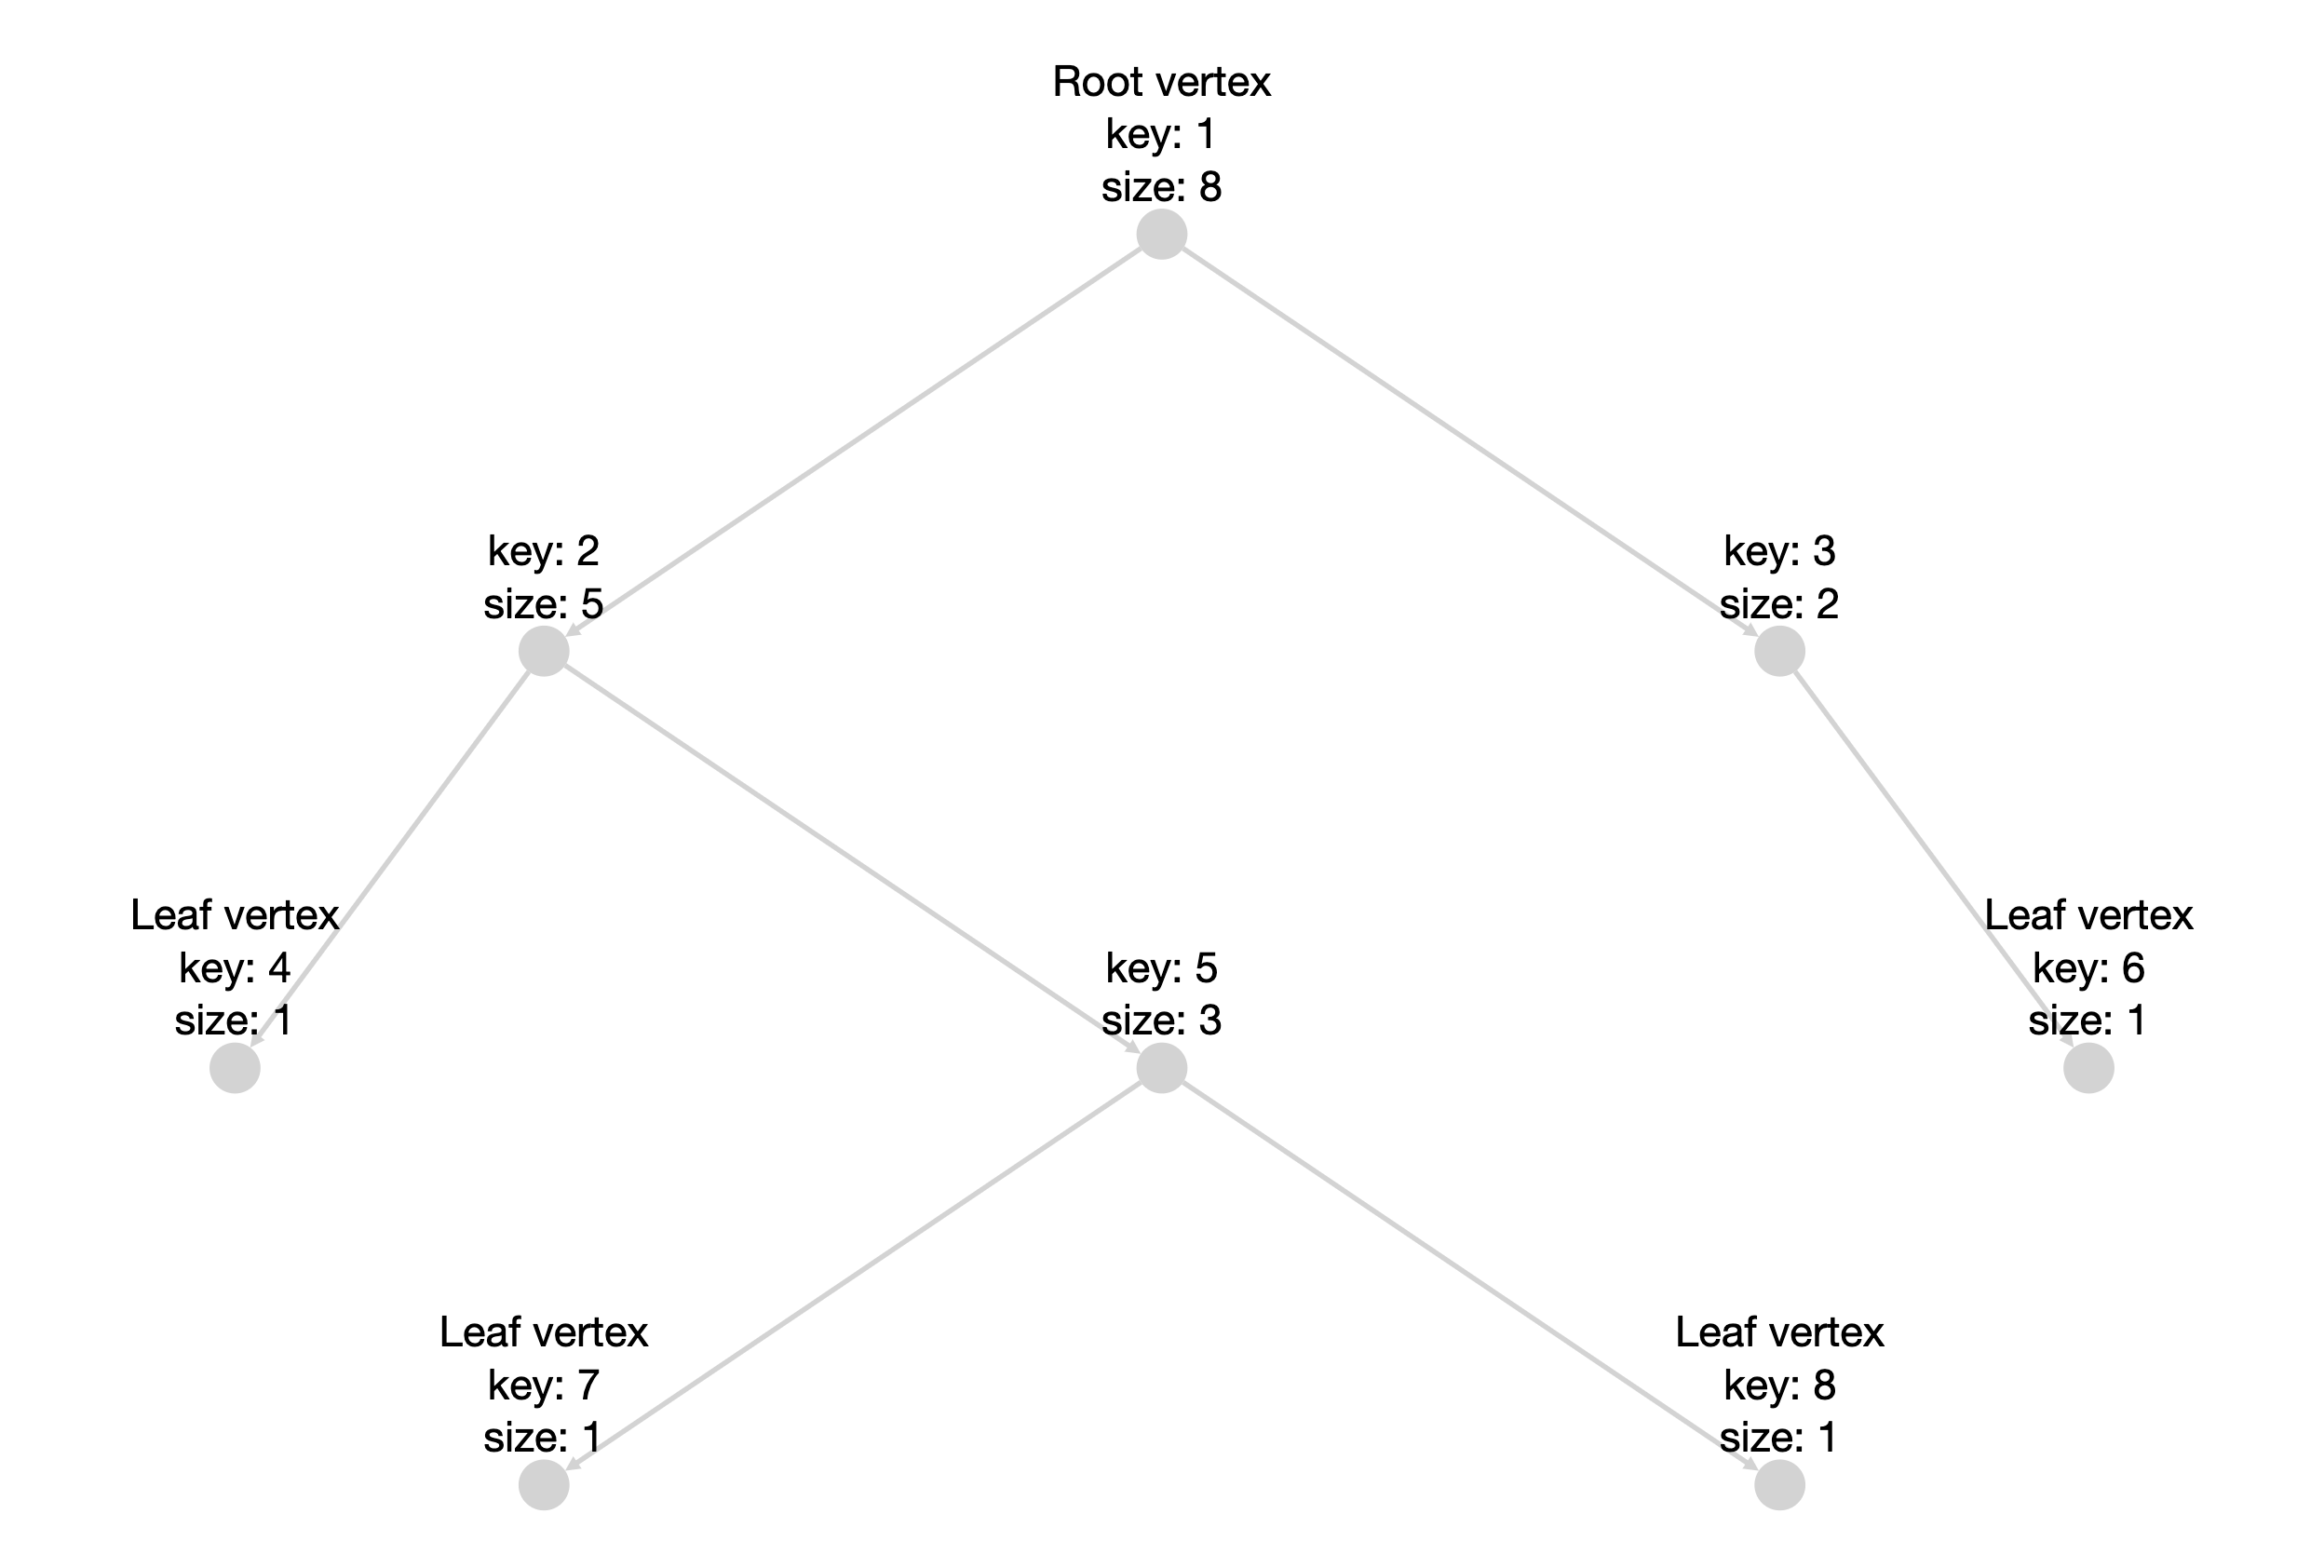
\includegraphics[scale=.175]{Fall23/p0_q1_BT_after.png}

 Your program should run in time $O(n)$ when given the root of a tree with $n$ vertices. In a sentence or two, informally justify why your program has such a runtime. 

\textbf{Solution}:
\begin{minted}{python}
    def calculate_sizes(v: Optional[BTvertex]) -> int:
        if v is None:
            return 0
        left = calculate_sizes(v.left)
        right = calculate_sizes(v.right)
        v.size = left + right + 1
        return v.size
\end{minted}

\begin{quote}
    \color{purple}
    The function dives to the bottom of the tree and climbs upward. At each level of the tree, a parent receives the sum of the left and right children and returns their sum. For a tree with n nodes, it takes roughly n steps to dive to the bottom of the tree and n steps to climb back up, which results in $O(n)$ time complexity. 
\end{quote}
 
 \item (proof warmup) \label{part:warmup}
 Removing a vertex \btv\ from a tree \treeT\ yields up to three disjoint trees: the subtree rooted at
 \texttt{v.left} (unless \texttt{v.left==None}), the subtree rooted at
 \texttt{v.right} (unless \texttt{v.right==None}), and a tree rooted at \texttt{T.root} consisting of all non-descendants of \btv\ (unless \texttt{T.root==v}).  For example:
 \\

 Before:
 
 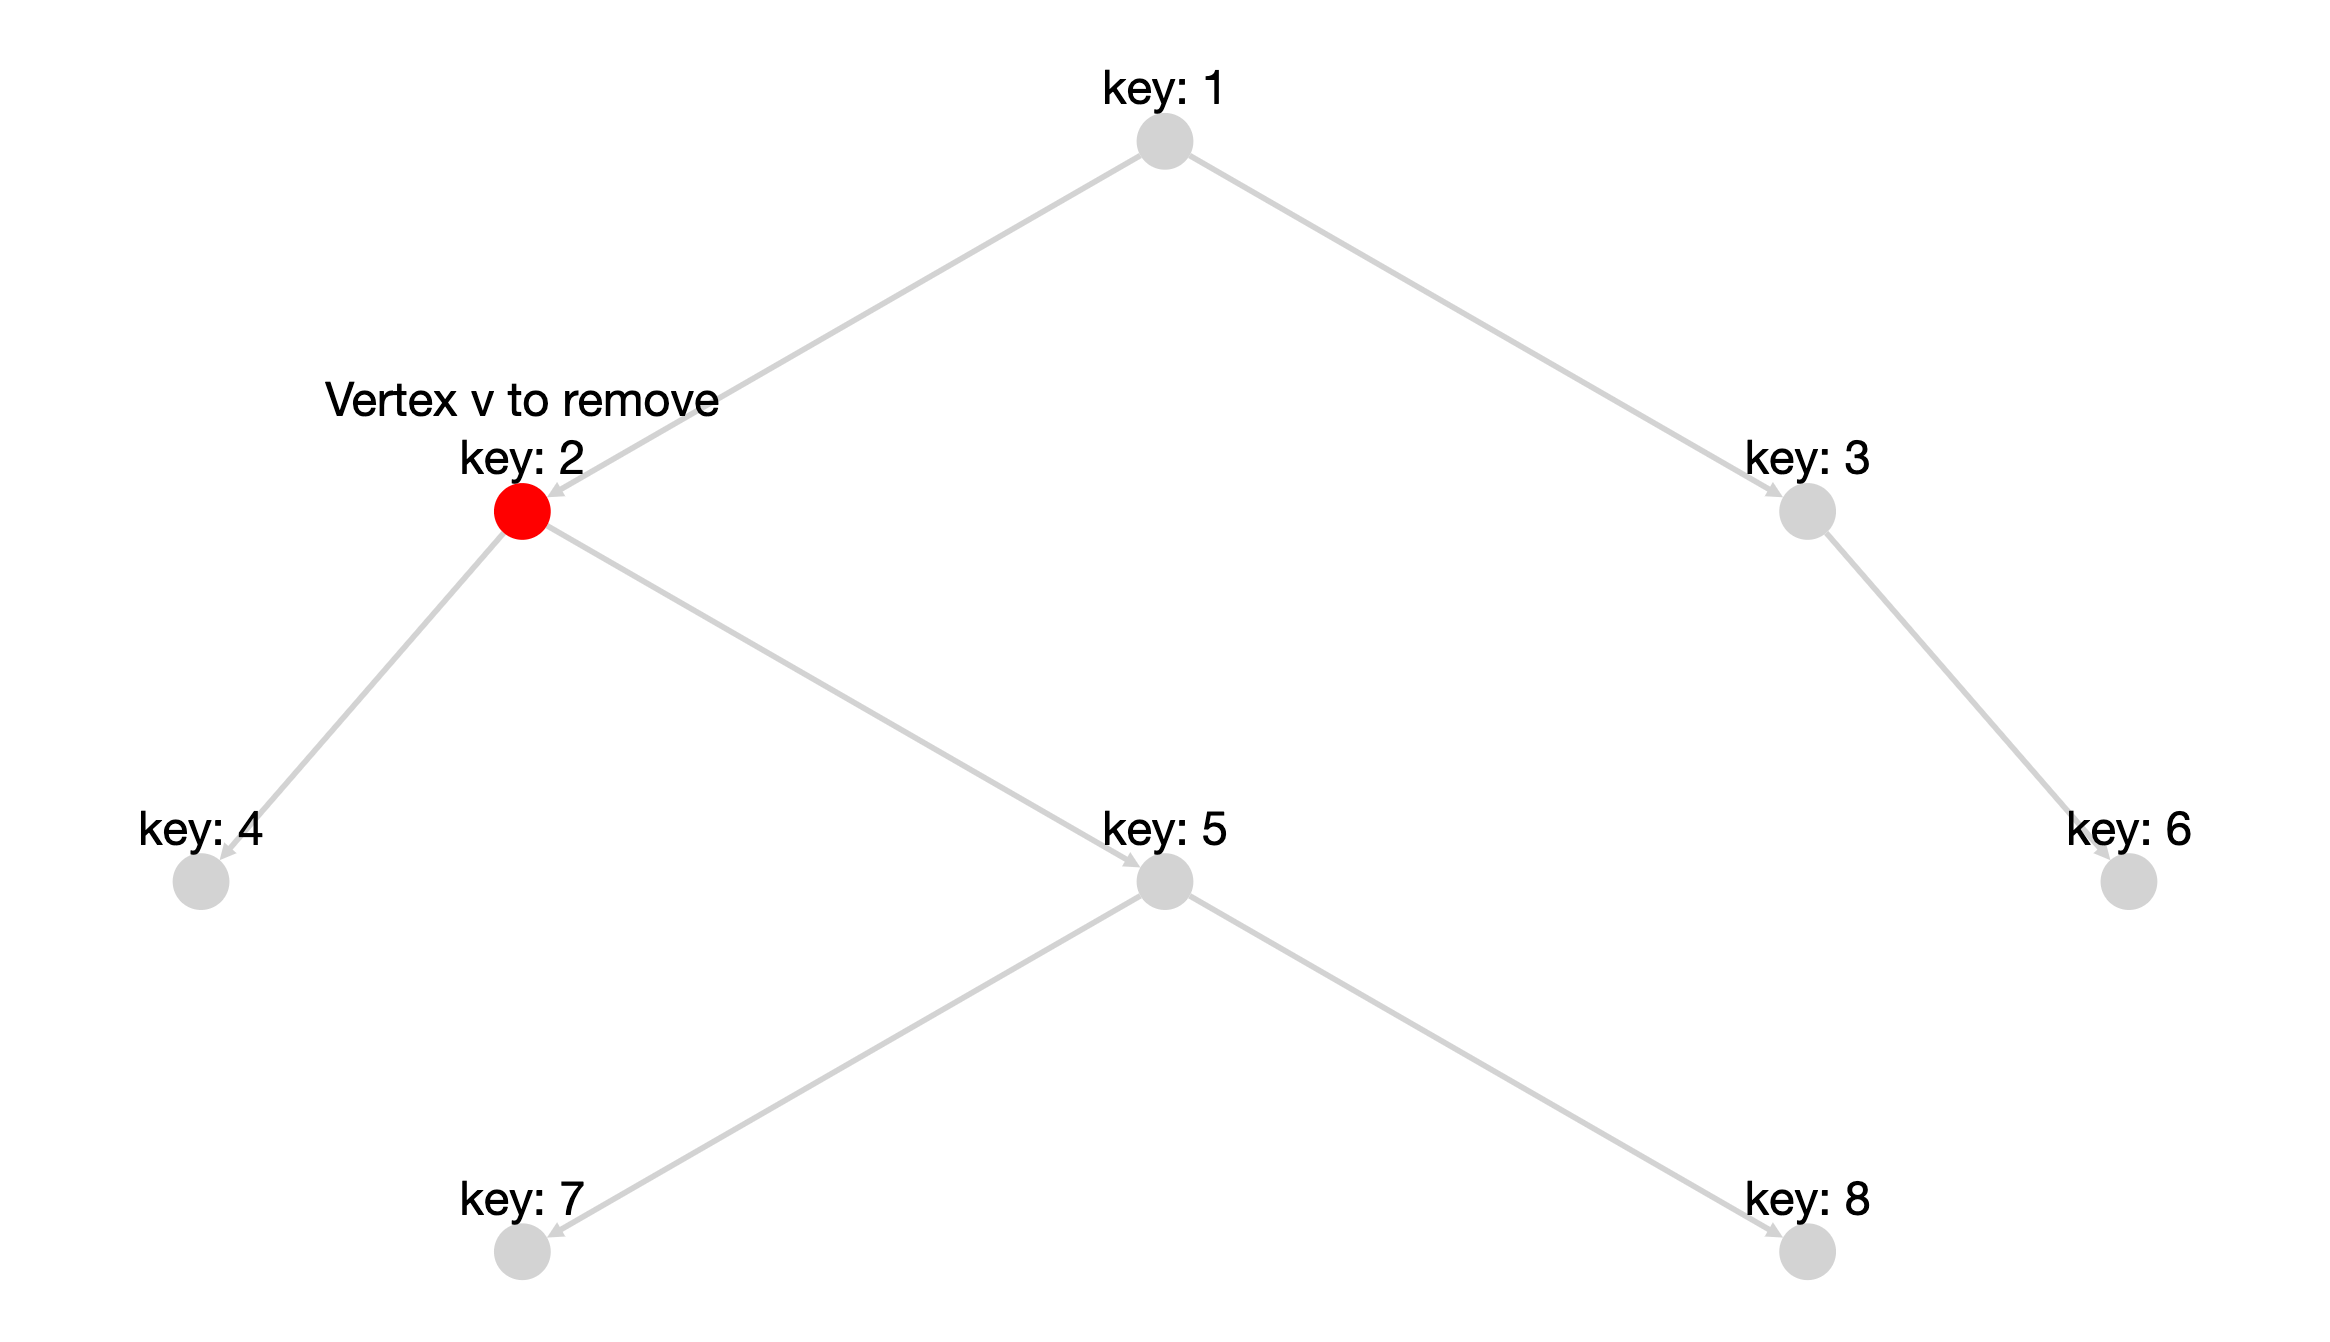
\includegraphics[scale=.175]{Fall23/p0_q1b_before.png}
 
 
 After:
 
  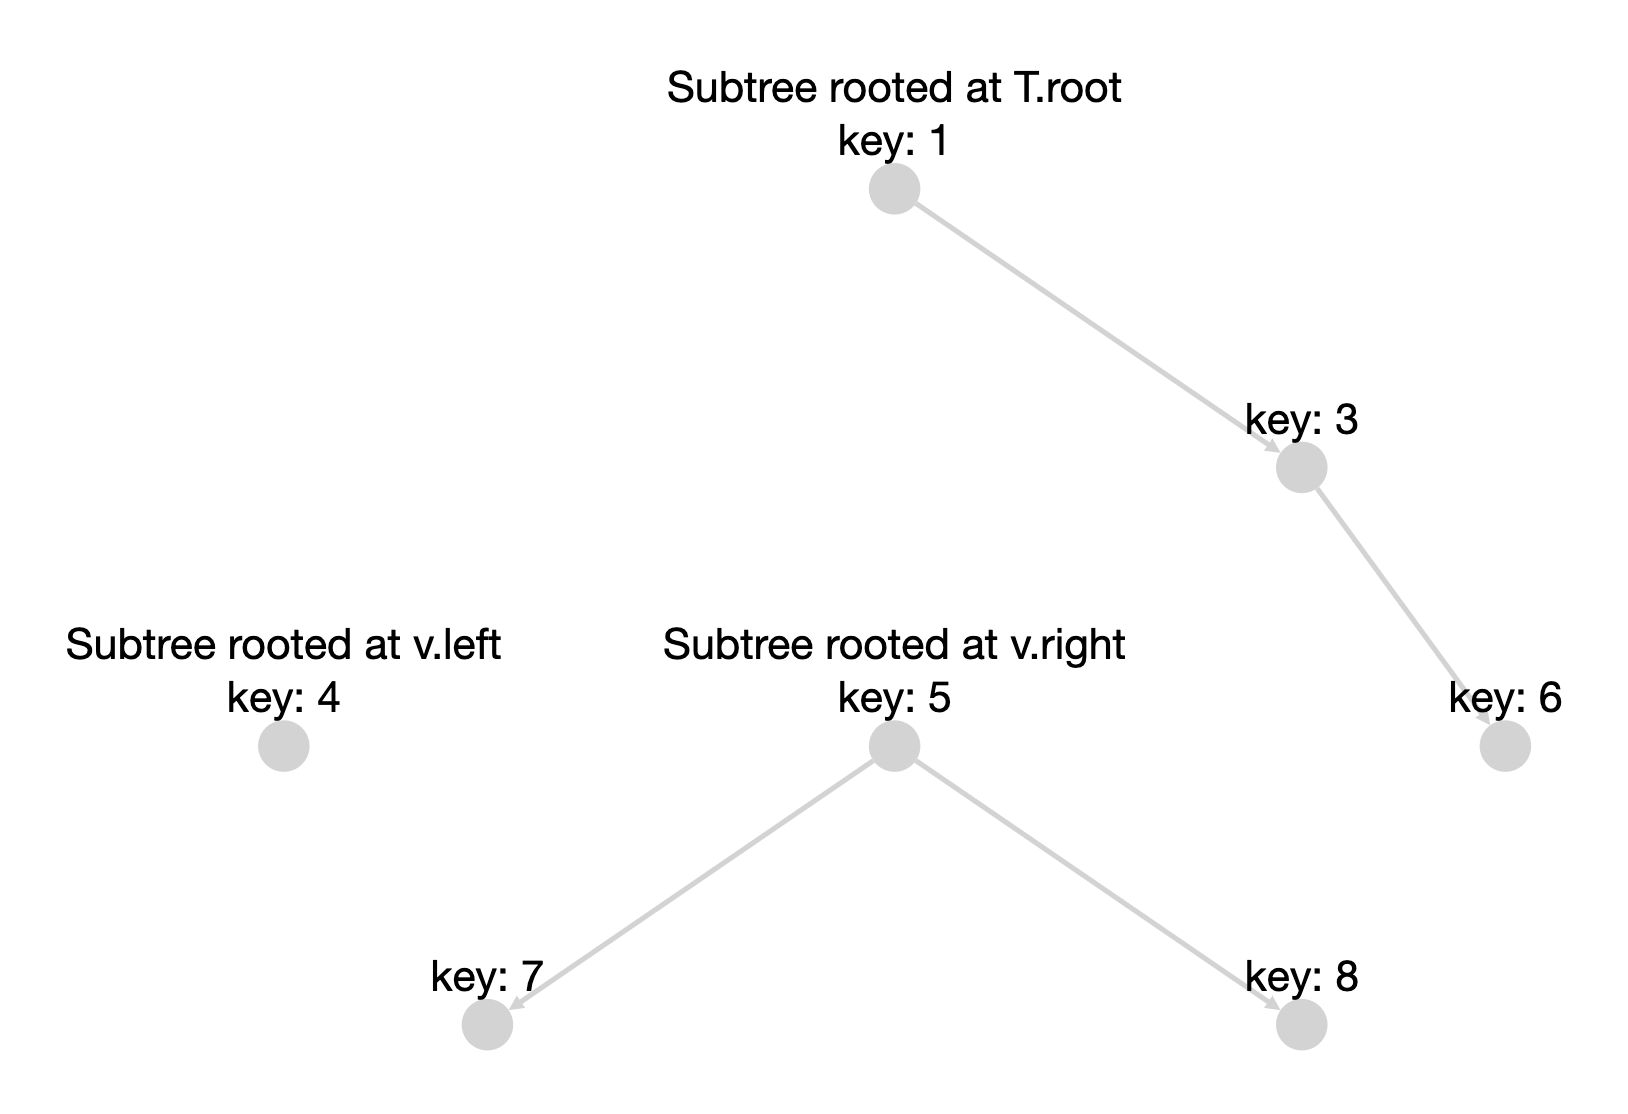
\includegraphics[scale=.225]{Fall23/p0_q1b_after.png}

  Suppose that for a vertex \btv, the largest subtree created by removing \btv\ contains a neighbor (i.e. child or parent) \btv$^*$\ of \btv\ and a total of $\phi(\btv)$ vertices (including \btv$^*$).
  If we remove \btv$^*$ and not \btv, we create at most two subtrees which don't contain \btv: prove that these subtrees each contain fewer than $\phi(\btv)$ vertices.

  \textbf{Solution}:
  \begin{quote}
    \color{purple}
    \textit{Direct proof}: Let $T$, $v$, $v$*, and $\phi$ be as defined above. \newline 
    If $v$* in the largest subtree not containing $v$ was the parent of $v$ before its removal, removing $v$* from $T$ instead produces one subtree not containing $v$. That subtree is either empty or contains a non-$v$ neighbor of $v$*. When $v$* is removed, the subtree of size $\phi(v)$ loses a leaf or root and has at most $\phi(v) - 1$ total vertices. \newline 
    If $v$* in in the largest subtree not containing $v$ was a child of $v$ before its removal, removing $v$* from $T$ instead produces two subtrees not containing $v$. These subtrees are either empty or rooted by children of $v$*. Without $v$* as a parent, the greatest of these child trees has at-most $\phi(v) - 1$ total vertices. \newline
    Because $\phi(v*)$ not containing $v$ is at-most $\phi(v) - 1$, all subtrees not-containing $v$ produced by removing $v$* from $T$ must have fewer than $\phi(v)$ vertices. 
\end{quote}

 \item (proofs by contradiction) \label{part:contradiction}
  Prove that in every tree \treeT\ of size $n$, there exists a vertex \btv\ such that removing \btv\ from \treeT\ results in disjoint trees that all have size at most $n/2$.  \\

  You may prove this however you like, but a recommended approach is to extend Part~\ref{part:warmup} and show that if the largest subtree created by removing a vertex \btv\ contains a neighbor \btv$^*$ of \btv\ and contains $\phi(\btv) > n/2$ vertices, then if we remove \btv$^*$ and not \btv, the subtree \emph{containing} \btv\ contains at most $n/2$ vertices. Then choose \btv\ to be the vertex for which $\phi(\btv)$, the size of the largest tree created by removing \btv, is smallest.

  \textbf{Solution}:
  \begin{quote}
    \color{purple}
    \textit{Proof by contradiction}: Assume for purposes of contradiction there exists some binary tree $T$ of size $n \in \mathbb{N}$ such that every vertex $v_k$, if removed, is guaranteed to produce at least one subtree of size $\phi(v_k) > \frac{n}{2}$. \newline
    Select some arbitrary vertex $v_0$ in $T$. If removed, at most three subtrees are produced. Let $v_1$ be a neighbor of $v_0$ and a member of the largest of those subtrees. By the assumed invariant of $T$, $\phi(v_0) > \frac{n}{2}$. \newline 
    Consider removing $v_1$ instead. By the proof above,  $\phi(v_0) \geq \phi(v_1) + 1$. Assuming the maximum value of $\phi(v_1)$, the inequality for $\phi(v_0)$ implies $\phi(v_1) + 1 > \frac{n}{2}$. Because $\phi(v_1)$ may be equal to $\frac{n}{2}$ and still satisfy this inequality, the invariant of $T$ is not maintained by $\phi(v_1)$. \newline
    If $v_0$ were removed, the maximum size of its lesser subtree would have been $n - \phi(v_0)$. Because $\phi(v_0) > \frac{n}{2}$, the maximum size of the lesser subtree would have been $\frac{n}{2} - 1$. If $v_1$ is removed instead, the size of the subtree now containing $v_0$ is at most $\frac{n}{2} - 1 + 1 = \frac{n}{2}$. This too fails to maintain the invariant of $T$. \newline 
    Because removing some $v_1$ on $T$ may produce a state that fails to preserve the claim about $T$, we can assume by contradiction that the claim was invalid and every tree of size $n$ has a vertex $v$ such that removing $v$ results in disjoint trees that all have size at most $\frac{n}{2}$.
\end{quote}

 \item (from proofs to algorithms)  Turn your proof from Part~\ref{part:contradiction} into a Python program that given a root vertex \texttt{r} of a {\em size-augmented} tree \treeT\ with $n$ vertices finds a vertex \btv\ with $\phi(\btv)\leq n/2$. Your program should run in time $O(h)$ on all size-augmented trees of height $h$; again informally justify why your program has such a runtime. (Hint: try to repeatedly reduce the potential function by moving to children. Why don't we need to try moving to parents as in the previous proof?)
\newpage
\textbf{Solution}:
\begin{minted}{python}
def find_vertex(r: Optional[BTvertex]) -> Optional[BTvertex]:
    if r is None:
        return r
    half = r.size // 2
    while r:
        if r.left and r.left.size > half:
            r = r.left
            continue
        if r.right and r.right.size > half:
            r = r.right
            continue
        return r
    raise Exception("failed to find a solution")
\end{minted}

\begin{quote}
    \color{purple}
    If any subtree of the current vertex has a child with size exceeding $\frac{n}{2}$, the breakpoint must be somewhere in that subtree. By descending the tree in such a way, the first vertex at which neither child exceeds $\frac{n}{2}$ is the target vertex. Because the function only ever moves downward and only ever visits a single node at any height in the tree, the runtime complexity is in terms of the height of the tree, $O(h)$.
\end{quote}
 
 \end{enumerate}
 
 \newcommand{\incomp}{\mathit{incomp}}
 \item (matchings and induction)
 Later in the course, we will study matching algorithms that are used in practice to match kidney donors to patients.  The challenge in general is that some donors are incompatible with some patients (i.e. the patient's body is likely to reject the donated kidney).  Suppose we are very lucky and have $n$ donors and $n$ patients where each donor $d$ is incompatible with exactly one patient, denoted $\incomp(d)$, and each patient $p$ is incompatible with exactly one donor $\incomp(p)$. (Incompatibility is symmetric, so $\incomp(d)=p$ iff $\incomp(p)=d$.)  Let $f(n)$ be the number of ways, under these circumstances, of matching donors to patients so that each donor donates exactly one kidney to a compatible patient and each patient receives exactly one kidney from a compatible donor.  


 \begin{enumerate} 
\item Show that for all $n\geq 3$,
 $$ f(n) > (n-1)\cdot f(n-2).$$
 Hint: let $d$ be one of the donors, and consider all possible patients $p$ with whom $d$ could be matched.  Then consider the case where $\incomp(p)$ is matched with $\incomp(d)$.

\begin{quote}
    \color{purple}
    In a sample of $n \geq 3$ patients, donors, and incompatibilities, let patient $p_k$ be incompatible with donor $d_k$ for $k \in \mathbb{N}, 0 \leq k < n$. \newline
    Arbitrarily select any patient. For example, $p_0$. There are initially $n - 1$ possible matches between $p_0$ and a donor. This is because $p_0$ can match with every donor except $d_0$. \newline 
    Say $p_0$ arbitrarily matches with $d_1$. After this match, one remaining patient and one remaining donor become able to match with anyone. In this example, $d_0$ is now compatible with every remaining patient, and $p_1$ is now compatible with every remaining donor. There are $n - 1$ patients and donors but fewer than $n - 1$ incompatibilities. Patient $p_1$ could feasibly match with $n - 1$ donors again instead of $n - 2$. This produces some nonzero surplus of matches over $f(n - 1)$, which we will call $x_n$. So, $f(n) = (n - 1) \cdot (f(n - 1) + x_n)$. \newline
    Place this in the given inequality and simplify: \newline
    \begin{align*}
        && (n - 1) \cdot (f(n - 1) + x_n) > (n - 1) \cdot f(n - 2) && \text{Substitute $f(n)$} && \\
        && f(n - 1) + x_n > f(n - 2) && \text{Divide common terms} &&  \\
        && (n - 2) \cdot (f(n - 2) + x_{n - 1}) + x_n > f(n - 2) && \text{Expand $f(n - 1)$} \\
        && (n - 2) \cdot f(n - 2) + (n - 2) \cdot x_{n - 1} + x_n  > f(n - 2) && \text{Multiply terms} && \\
        && (n - 2) \cdot x_{n - 1} + x_n > f(n - 2) - (n - 2) \cdot f(n - 2) && \text{Move $f(n - 2)$} && \\
    \end{align*}
    Because $n \geq 3$, the right side of the final inequality is at most 0. Because $x_{n - 1}$ is at least $1$, the left side of the inequality is at least 1. So, the inequality is valid.
\end{quote}

 \item
 In fact, show that for all $n\geq 3$, we have
 $$ f(n) = (n-1)\cdot (f(n-1)+f(n-2)).$$
 This will require you to include the remaining case where $\incomp(p)$ is \emph{not} matched with $\incomp(d)$, unlike the previous exercise.

\begin{quote}
    \color{purple}
    Extending the variables and reasoning above, recall that $f(n)$ represents the number of possible matches in the presence of $n$ patients, donors, and incompatibilities. After the first match, there's one donor and one patient who can match with any other donor and any other patient. \newline 
    If we treat these "free agent" members as if they actually had an associated incompatibility, we'd again have equal patients, donors, and incompatibilities among an $n - 1$ sized sample, which we know has $f(n - 1)$ matches. \newline
    If instead, however, the free donor and patient immediately match with each other, there are now $n - 2$ patients, donors, and incompatibilities, which we know has $f(n - 2)$ matches. \newline
    Because these two events may happen for any match in the initial sample of $n$, we can conclude that $f(n) = (n - 1) \cdot (f(n - 1) + f(n - 2))$.
    
\end{quote}

 \item 
 Prove by strong induction that for all $n\geq 2$,
 $$\frac{n!}{3} \leq f(n) \leq \frac{n!}{2}.$$
 
\begin{quote}
    \color{purple}
    \textit{Proof by strong induction}:
    \item \textit{Base case 1}: $n = 2$.
    \begin{itemize}
        \item $\frac{2!}{3} = \frac{2}{3}$
        \item $f(2) = 1$. With two patients, donors, and incompatibilities, each patient can match once with the single donor they are not incompatible with.
        \item $\frac{2!}{2} = 1$
        \item Because $\frac{2}{3} \leq 1 \leq 1$, this case holds.
    \end{itemize}
    \item \textit{Base case 2}: $n = 3$
    \begin{itemize}
        \item $\frac{3!}{3} = 2$
        \item $f(3) = 2$. $f(1) = 0$ because a single patient and single donor are incompatible. Applying the formula from 2c, $f(3) = 2 \cdot (f(2) + f(1)) = 2 \cdot 1 = 2$. 
        \item $\frac{3!}{2} = 3$
        \item Because $2 \leq 2 \leq 3$, this case holds.
    \end{itemize}
    \textit{Inductive hypothesis}: Let $k$ be some natural number greater than $2$. Assuming the inequality is valid for $k - 1$ and $k$, prove the inequality holds for $k + 1$: \newline \newline
    Leveraging the definition of factorial, at $k + 1$, the inequality can be expressed and simplified as below: 
    \begin{align*}
        && \frac{k!}{3} \cdot (k + 1) \leq k \cdot (f(k) + f(k - 1)) \leq \frac{k!}{2} \cdot (k + 1) && \text{Apply formulas} && \\
        && \frac{k! \cdot k}{3} + \frac{k!}{3} \leq k \cdot f(k) + k \cdot f(k - 1) \leq \frac{k! \cdot k}{2} + \frac{k!}{2} && \text{Distribute} && \\ 
        && \frac{k!}{3} + \frac{(k - 1)!}{3} \leq f(k) + f(k - 1) \leq \frac{k!}{2} + \frac{(k - 1)!}{2} && \text{Divide by $k$} && \\
    \end{align*}
    By the inductive hypothesis, we can assert that $\frac{(k - 1)!}{3} \leq f(k - 1) \leq \frac{(k - 1)!}{2}$ is true and $\frac{k!}{3} \leq f(k) \leq \frac{k!}{2}$. The final inequality above is simply the sum of two already-known valid inequalities, so we can assert that the derived inequality is valid. Thus, through strong induction, we know that $\frac{n!}{3} \leq f(n) \leq \frac{n!}{2}$ for all $n \geq 2$.
\end{quote}
 \end{enumerate}



\end{enumerate}


\end{document}
